% !TEX encoding = UTF-8 Unicode
% !TEX program = pdflatex
% !TEX spellcheck = en_US


% In order to correctly compile this document,
% execute the following commands:
% 1. pdflatex
% 2. pdflatex
% 3. pdflatex



\documentclass[amsthm,ebook]{saparticle}

% IF YOU USE PDFLATEX
\usepackage[utf8x]{inputenc}
% if you write in english and in greek
\usepackage{ucs}
\usepackage[greek,english]{babel}
\languageattribute{greek}{polutoniko}

% IF YOU USE XELATEX
%\usepackage{polyglossia}
% if you write in italian
%\setmainlanguage{italian}
% If you want put some ancient greek:
%\setotherlanguage[variant=polytonic]{greek}
%\newfontfamily{\greekfont}[Ligatures=TeX]{Palatino Linotype}

% dummy text (remove in a normal thesis)
% remove if not necessary
\usepackage{siunitx}
%Natbib for bibliography management
\usepackage[authoryear]{natbib}
% custom commands
\newcommand{\bs}{\textbackslash}

%%%%%%%%
%TITLE:%
%%%%%%%%
\title{Epigraphy and onomastics in the Hesperia databank}
\author[barc]{Noemí Moncunill Martí \corref{first}}
\author[sorb]{Javier Velaza}
\address[sorb]{Université de Paris-Sorbonne (Paris IV)}
\address[barc]{University of Barcelona2}
\cortext[first]{Corresponding author. Email: nmoncunill@gmail.com}
\date{2015-11-15}
\begin{document}

\maketitle
\begin{abstract}
The first part of this work provides a general overview of the features and advantages of the digital epigraphic corpora
on the basis of the experience gained in the last years within the Hesperia project. The second part of the paper
provides a detailed presentation of the new sections available in the Hesperia databank devoted to indigenous personal
names and divinity names.
\end{abstract}
\keywords{Hispania, epigraphy, onomastics, digital corpora, Palaeohispanic languages and writings}


\section{Introduction}


\noindent The aim of this work is to do a general overview of the computer-based epigraphic corpora, to think about their features
and advantages, taking the experience gained in the last years within the Hesperia project as a starting point.\footnote{ This paper is an output from the FFI2012-25113 project and the Senior Research Team LITTERA
(2014SGR63), on the one hand, and 655938 — ZEPHYROS — H2020-MSCA-IF-2014 project, on the other.}

The first thing that necessarily needs to be highlighted is that traditional epigraphic corpora have certain limits that
are imposed by their morphology and format. If summarizing, there are three main and most evident limitations: 
\begin{description}
\item[a] One-dimensional format. The monument's description, the textual edition, the critical apparatus and remarks are
displayed one after another, with no wider possibility to link one to another than through some indices, which by the
way are rarely detailed enough. Not even in the most extended indices, as those in CIL, the connexions between
inscriptions through such relevant data as their date, palaeography or onomastics are set clear. Obviously, those
connexions can be set by the users in their mind, but when the corpus displays thousands or tens of thousands of
inscriptions, it looks too optimistic to take for granted that most readers will have the aptitude such work takes.

\item[b] Ephemeral usefulness. It looks also obvious that a traditional corpus will necessarily be always ephemeral for many
reasons: new inscriptions cannot be added, mistakes cannot be corrected, text editions cannot be improved and
modifications based on new evidence or knowledge cannot be introduced, among other limitations. Of course some of these
problems have hardly been solved by publishing some supplements, but it is widely known that these are partial
solutions only.

\item[c] Authoritative work. In a traditional corpus, editors impose their knowledge in a large range of features, and thus
they interfere in the utility of other views, to the extent of depreciating them too much. When it comes to an
epigraphic corpus that is written in a wide-known language, such as Latin, this auctoritas becomes particularly
powerful regarding the reading of the epigraphic text, its checking being not possible all the time for users,
particularly for those who are not experts on the subject. But when it comes to fragmentary languages, with very low or
even no language deciphering at all, and with many doubts on decoding, the truth is that the influence of the editor is
extremely high and involves some risks that they do not always come to terms with successfully.


\end{description}
In our opinion, these limitations can be solved or, at least, diminished by a proper and efficient use of the tools IT
puts to our disposal. Although this is no longer anything of new, any attempt to use them so far has brought to an
output too close to the traditional, non-innovative epigraphic corpora, considering the features of such new tools. To
get over one-dimensional formats, an open, adaptable digital structure must be created that shall take the most out of
every single datum in the database. Besides, getting over an ephemeral usefulness requires the possibility not just to
keep adding new data, but also to connect the database with any other tool with a similar structure and to extend the
platform with any new or advisable features. Finally, the authoritative temptation must be also avoided, particularly
through systems that shall bring to users the possibility to take their own decisions in certain issues of an open
debate and, at the end of the day, to customize their own corpus.

Along with the above-said, some other advantages any digital edition shall bring must be taken into account, although it
looks unnecessary to discuss them: for instance, an online building of the corpus shall allow cooperation and
simultaneous work of interdisciplinary teams that will not only contribute to speed up the work and check the
achievements, but also to enrich the views in such studies and the analysis of the monuments and their texts. The
open-access format of the corpus means also a big leap for research in this field, along with an important service of
transferring knowledge to society. However, it must be recalled that every corpus shall be adapted to the specific
features of the documents and their epigraphic culture (and other sources, eventually) has left to us. And such terms
require a constant dialogue between epigraphists and technicians since the very beginning of the project, in spite of
the fact that they do not always come to understand each other. Those projects that had any of these groups prevailing
at the start of the project have proved to have insuperable lacks through their stages. 

\section{The Hesperia project}


\noindent All above-mentioned principles have been taken into account in Hesperia project, its main goal being to gather all
linguistic evidences from Palaeohispanic languages, that is, pre-Roman languages in the Iberian Peninsula\footnote{
General presentations of the project can be found in \citet{orduna_implementing_????}, \citet{orduna_philology_????} and
\citet{velaza_hesperia:_2014}.}. First of all, we need to recall these are very different materials as for their quantity, quality and
reliability. Ancient Hispania left us epigraphic texts in at least four languages: Tartessian, Iberian, Celtiberian and
Lusitanian -{}-the possibility there are also some texts in Palaeobasque language is still sub iudice\footnote{
Concerning this subject, see \citet{velaza_epigrafiy_2009}.}{}-{}-, mainly written in four epichoric scripts -{}-Tartessian,
southeastern-Iberian, northeastern-Iberian and Greek-Iberian script. 

\begin{figure}[!bp]
\centering
 \includegraphics[width=\columnwidth]{EpigraphyandonomasticsinHesperiadatabanktemplate-img001.jpg}
\caption{ Map of the Palaeohispanic inscriptions attested in the Iberian Peninsula.}
\label{fig:1}
\end{figure}


The current knowledge of each of these scripts is in very different stages, just as when it comes to their languages
deciphering. Along with the epigraphic texts there are also other evidences, as those from onomastics -{}-anthroponymy
and theonymy preserved in Roman inscriptions found in these territories, and toponymy from Classic sources-{}- and some
notes transmitted by several authors. 

Hesperia was born as a natural successor in the digital era of the main corpus for Palaeohispanic languages, that is
Monumenta linguarum Hispanicarum, published between 1975 and 2001 by Jürgen Untermann. The project conception is due to
Javier de Hoz and its digital platform has mainly been developed by Eduardo Orduña. Nowadays it is coordinated by an
interdisciplinary and interuniversity team with researchers from the Universidad Complutense de Madrid, the Universidad
del País Vasco, the Universidad de Zaragoza and the Universidad de Barcelona. There are currently several sections open
for searching (\url{http://hesperia.ucm.es/}).

\begin{figure}[!bp]
\centering
 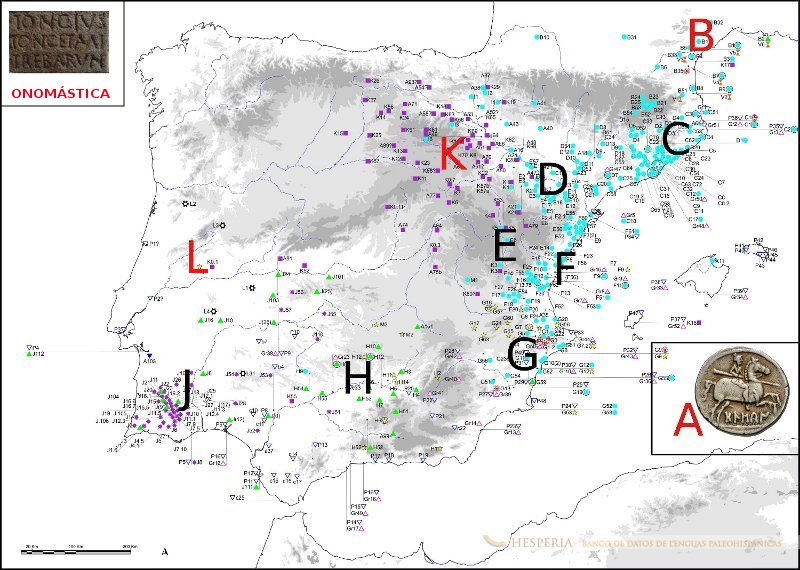
\includegraphics[width=\columnwidth]{EpigraphyandonomasticsinHesperiadatabanktemplate-img002.png}
\caption{Dispersal areas of Palaeohispanic inscriptions and sections available in Hesperia databank}
\label{fig:2}
\end{figure}

\begin{description}
\item[i] Partial epigraphic corpora from B zone (Iberian inscriptions from the south of France), K zone (Celtiberian
inscriptions) and L zone (Lusitanian inscriptions). All of them follow the same data form made of six tabs
corresponding to ``general features'', ``text'',
``epigraphy and paleography'', ``pictures'',
``arqueological context'' and ``bibliography''. The databases are
linked between them through a powerful engine for simple and complex searches, and pdf documents as well as maps can be
created with the resulting outcomes. Work is currently being focused on C and D zones (Iberian inscriptions in
Catalonia), which is scheduled to be open for search by the end of 2015.

\item[ii] A numismatic database with its specific four-tab structure: ``general features'',
``inscription'', ``language and writing'' and
``bibliography'', where all Paleohispanic mints are gathered, no matter their scripts or
languages.

\item[iii] An onomastic database, with a specific search engine allowing combined searches with any of the elements typical
from the identified onomastic formulae. 

\end{description}

Beyond finishing, checking and updating the already-open sections, the team currently works on transversal fields, such
as lexicon, as well as on creating several kinds of tools, as the possibility of displaying the corpus according to
alternative readings -{}-which turns out to be essential in epigraphic contexts with a lower level of decoding, as in
Tartessian, although its applicability to other fields is still being tested-{}-. 

Besides, the team has also decided to consider the potential applicability of this corpus structure to other cultures of
the western Mediterranean. With such aim, prof. Francisco Beltrán leads the AELAW project (Ancient European Languages
and Writings), with the participation of researchers from ten different countries, and that has been granted a COST
program in order to build in future a single corpus with the evidences from all fragmentary languages documented in the
western Mediterranean for the Ancient times.

\section{The new sections on onomastics}


\noindent The Hesperia databank has been recently extended with a new resource on indigenous onomastics. More specifically, the
new sections now available are devoted to the anthroponymy and theonymy, leaving for the near future the data referring
to toponymy and ethnonymy, which are not yet available in open access.

In this new section we have compiled all the pre-Roman personal names and divinity names attested both by direct and
indirect tradition. This represents, so far, a total of nearly 6.000 records. Names attested in direct sources are
those that can be identified in epicoric epigraphies; the second group, in its turn, contains the names that can be
identified in the so-called colonial epigraphy, as well as in literary sources. Regarding the chronology of the
epigraphic material, the oldest texts are the Iberian, which can be dated back to the 5th century BC, whereas the most
recent ones are the Latin inscriptions from the high-imperial age. Thus, the processed information can be classified
into one of these groups:

\begin{itemize}
\item Indigenous names in Iberian inscriptions
\item Indigenous names in Celtiberian inscriptions 
\item Indigenous names in Lusitanian inscriptions
\item Indigenous names in Greek inscriptions
\item Indigenous names in Latin inscriptions
\item Indigenous names in ancient authors
\end{itemize}
The Greek and Latin epigraphy group mainly contains inscriptions from the Iberian Peninsula; nevertheless there are also
a few exemplars coming from outside this territory, but which clearly refers to individuals of Palaeohispanic origin.
The most significant document that fits into this category is the Ascoli bronze, which displays a long list of Iberian
equites to which the Roman citizenship was given. As a matter of fact, this artefact has become the most important
document for the study of Iberian personal names.

As said above, the database contains about 6.000 records so far; each of them reports a divinity name and/or the whole
onomastic formula of individuals whose complete name presents at least one indigenous element. This means that each
item is devoted to a concrete person, whose onomastic formula might be composed by several indigenous names. The
information of each record is completed with a bibliographical apparatus, and the find-spot coordinates, together with
a map. Moreover, the database allows using this geographic information to create new linguistic maps, which represents
one of the main strengths offered by this new tool of the Hesperia databank.

The following could be a good example of one of the above-described records. This Latin inscription from southern Spain
mentions a woman with a Latin nomen, Aelia, followed by an Iberian cognomen, Belesiar, as well as the name of an
indigenous divinity, Betatun. Thus, a single table records an indigenous personal name together with an indigenous god.
The lower part is reserved for the bibliographical references, the geographic information and, last but not least, the
map.

\begin{figure}[!bp]
\centering
 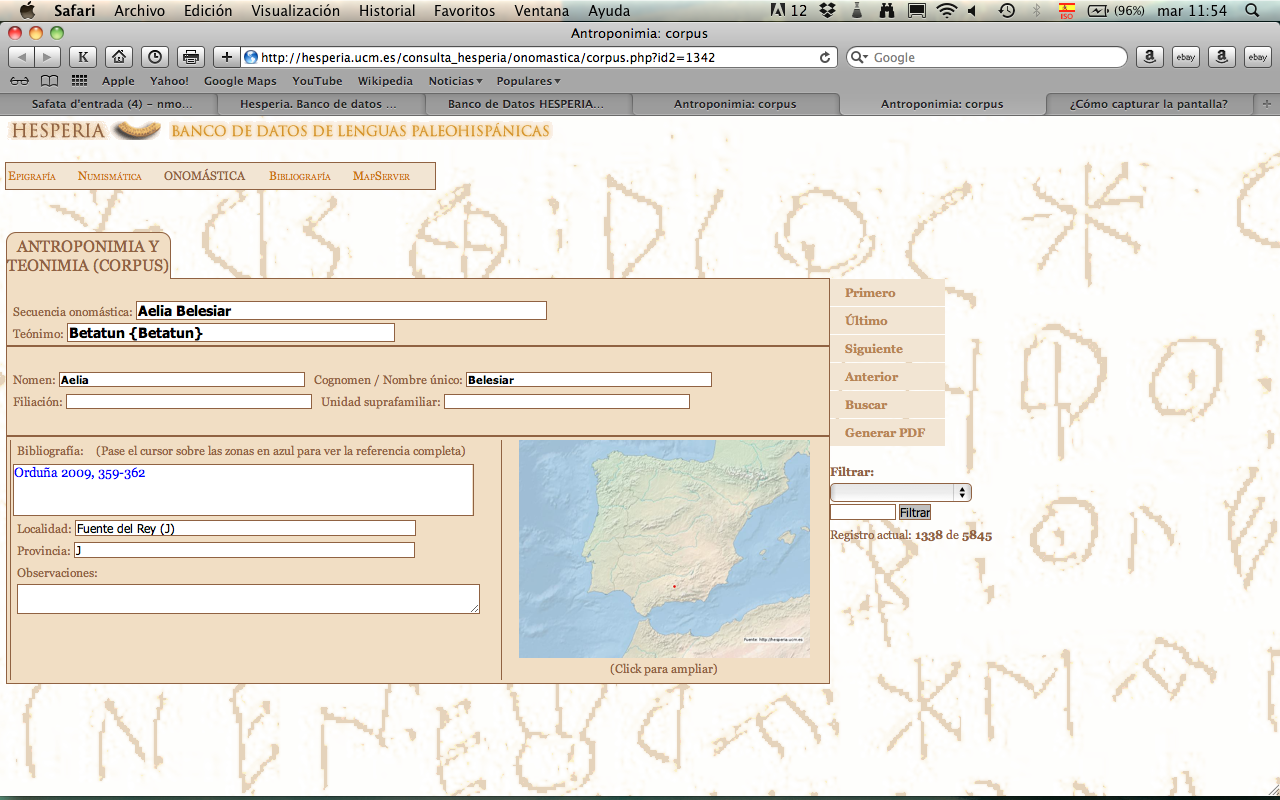
\includegraphics[width=\columnwidth]{EpigraphyandonomasticsinHesperiadatabanktemplate-img003.png}
\caption{Personal-names and divinity-names record in Hesperia databank.}
\label{fig:3}
\end{figure}

A slightly different kind of record is conceived to compile the personal names attested in literary sources. As shown
below, in these cases the bibliographical field is merely used to mention the ancient passages in which the name is
attested; there is no geographical information, and the “observations” field is often used just to report the different
graphical variants of the name.

\begin{figure}[!bp]
\centering
 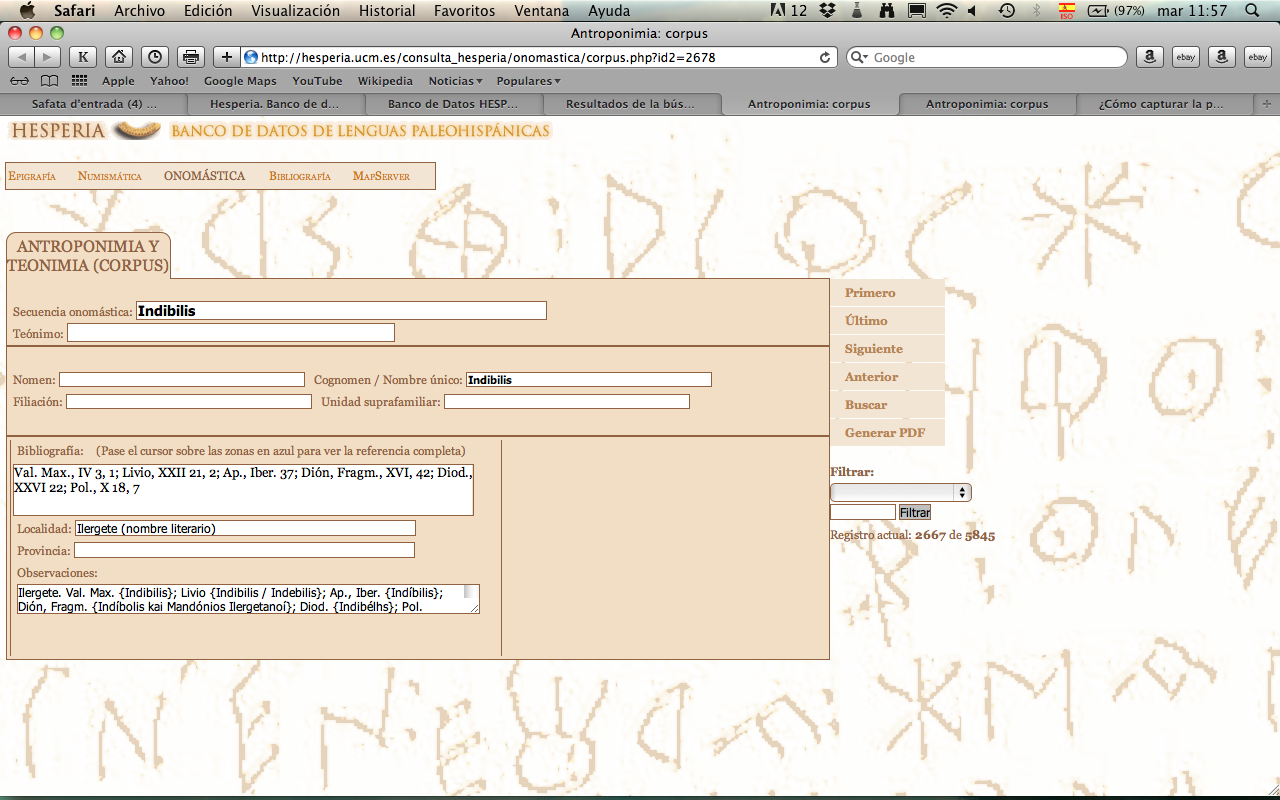
\includegraphics[width=\columnwidth]{EpigraphyandonomasticsinHesperiadatabanktemplate-img004.png}
\caption{Personal-names and divinity-names record in Hesperia databank.}
\label{fig:4}
\end{figure}

The goal of Hesperia is to provide, in the first place, an exhaustive repertory of all the Palaeohispanic names. Thus,
with the information available a map can be easily generated with all the spots where at least an indigenous name is
attested (in green); or a divinity name (in blue); or, finally, combine those maps in a single interactive map (in
green and blue), where each point is directly linked with the corresponding records.

\begin{figure}[!bp]
\centering
 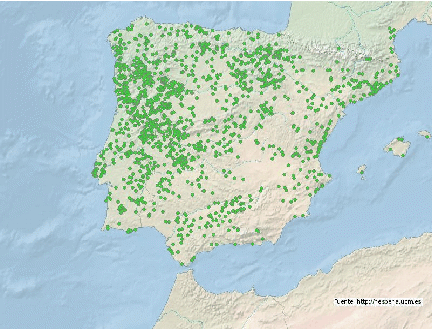
\includegraphics[width=\columnwidth]{EpigraphyandonomasticsinHesperiadatabanktemplate-img005.png}
\caption{Dispersal area of indigenous personal names.}
\label{fig:5}
\end{figure}


\begin{figure}[!bp]
\centering
 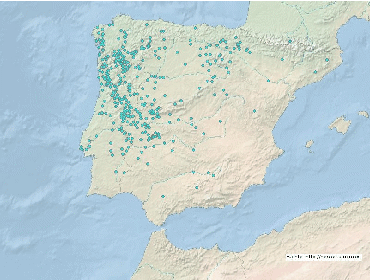
\includegraphics[width=\columnwidth]{EpigraphyandonomasticsinHesperiadatabanktemplate-img006.png}
\caption{Dispersal area of indigenous divinity names}
\label{fig:}
\end{figure}


\begin{figure}[!bp]
\centering
 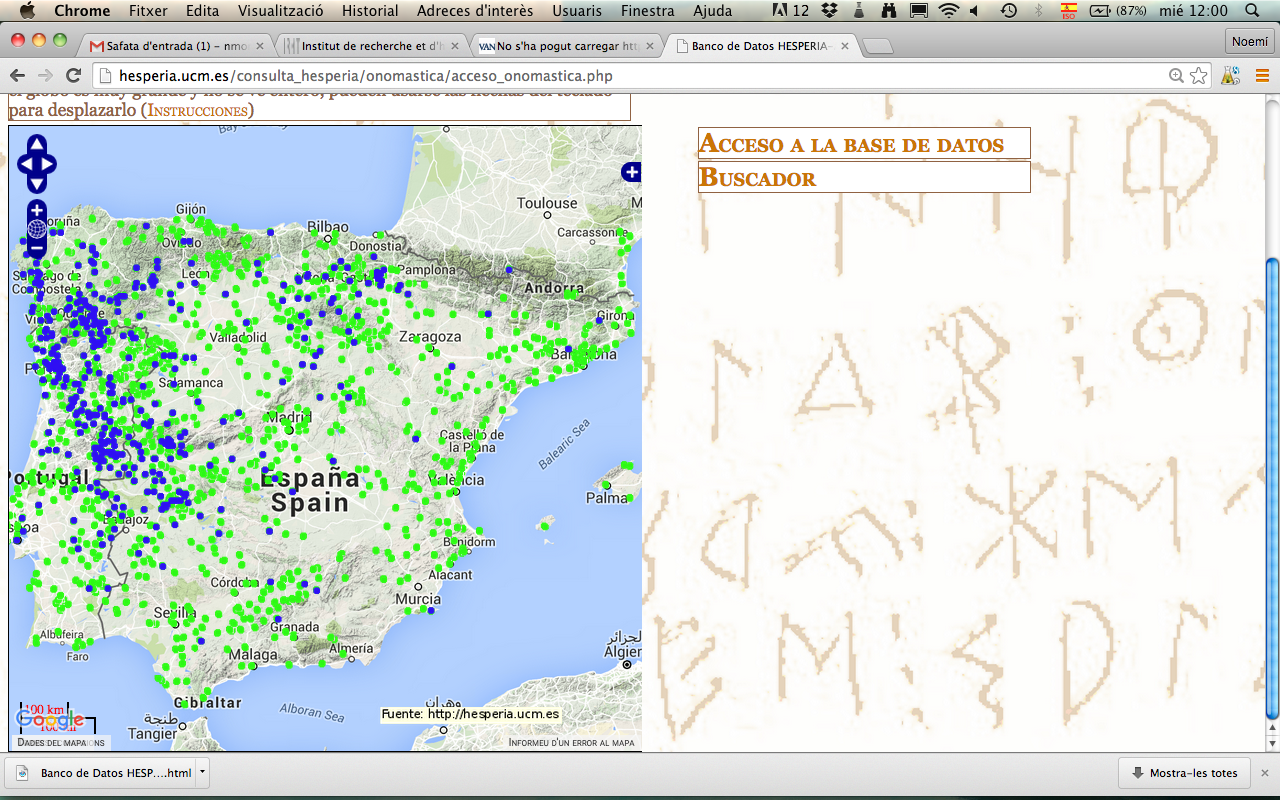
\includegraphics[width=\columnwidth]{EpigraphyandonomasticsinHesperiadatabanktemplate-img007.png}
\caption{Disperal areas of indigenous divinity names and personal names}
\label{fig:7}
\end{figure}
 

Thanks to the search engine, all these points can then be redistributed into smaller groups to draw linguistic areas or
isoglosses, on the basis, for instance, of the attestation of a well-known anthroponymic element or the dispersal area
of significant phonetic features. In the following maps it is displayed, in the first place, the attestation area of
names containing the element \emph{biur}, which clearly corresponds to the Iberian area, that is, the non indo-European half
of the Iberian peninsula; and, in the second place, it is displayed the dispersal area of the name Tancinus, which
clearly corresponds to the indo-European part.

\begin{figure}[!bp]
\centering
 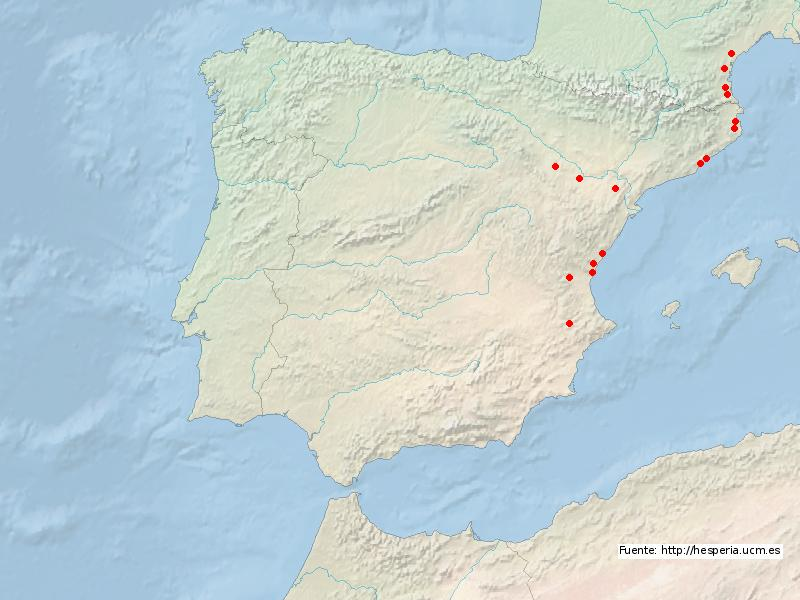
\includegraphics[width=\columnwidth]{EpigraphyandonomasticsinHesperiadatabanktemplate-img008.jpg}
\caption{Dispersal area of the anthroponymic element \emph{biur}}
\label{fig:}
\end{figure}


\begin{figure}[!bp]
\centering
 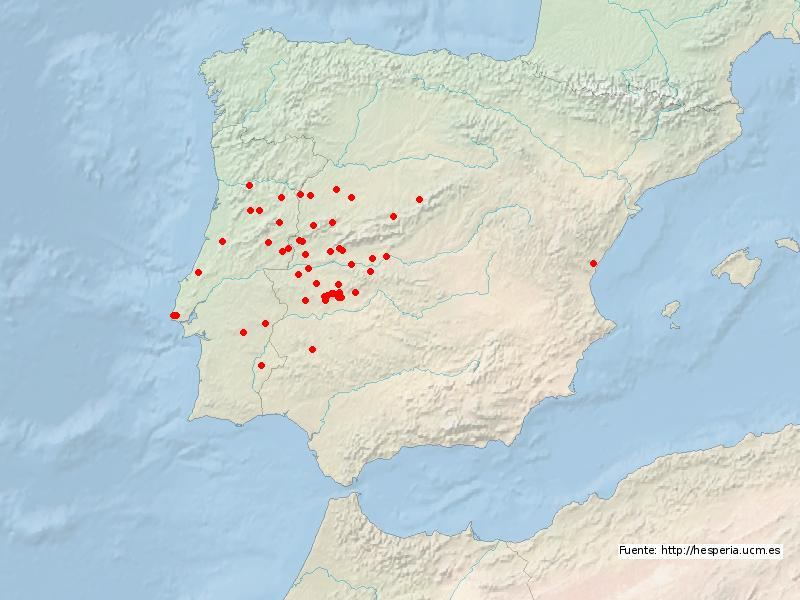
\includegraphics[width=\columnwidth]{EpigraphyandonomasticsinHesperiadatabanktemplate-img009.jpg}
\caption{Dispersal area of the name Tancinuse}
\label{fig:9}
\end{figure}


It must be pointed out that the Hesperia project is, in general terms, following the main standards for epigraphic
databanks and text editing, and we are now exploring ways to interact with the linked open data ecosystem (tagging
persons for compatibility with SNAP, places for compatibility with Pelagios/Pleiades, text references for compatibility
with IDEs, citations with CTS, object metadata with EAGLE, etc.).\footnote{ We thank Gabriel Bodard for his
observations at this regard.} 

The example below could provide an easy way to show to what extent the interrelationship between different open-access
databanks might be useful even in the present stage of the Hesperia project, where prosopography and toponymy have not
yet been fully developed. 

The following file contains information on a person’s or god’s name observed in an Iberian rock inscription in the
Pyrenees. Nevertheless, the structure of the word as well as its phonetic features show no possible interpretation in
Iberian. In consequence, other possibilities have to be considered, such as it could actually be an adaptation of a
Greek name. As a matter of fact, the same name is attested as a mythological character in literary sources (Parthenius
of Nicaea XXX 1; Ovid, Ibis 434), as well as record as a personal name in open-access databanks such as LGPN
(V5a-20577) or Trismegistos (Per 222620). Therefore, in this particular case, the linking between open-access data
could be helpful for the linguistic analysis itself.


\begin{figure}[!bp]
\centering
 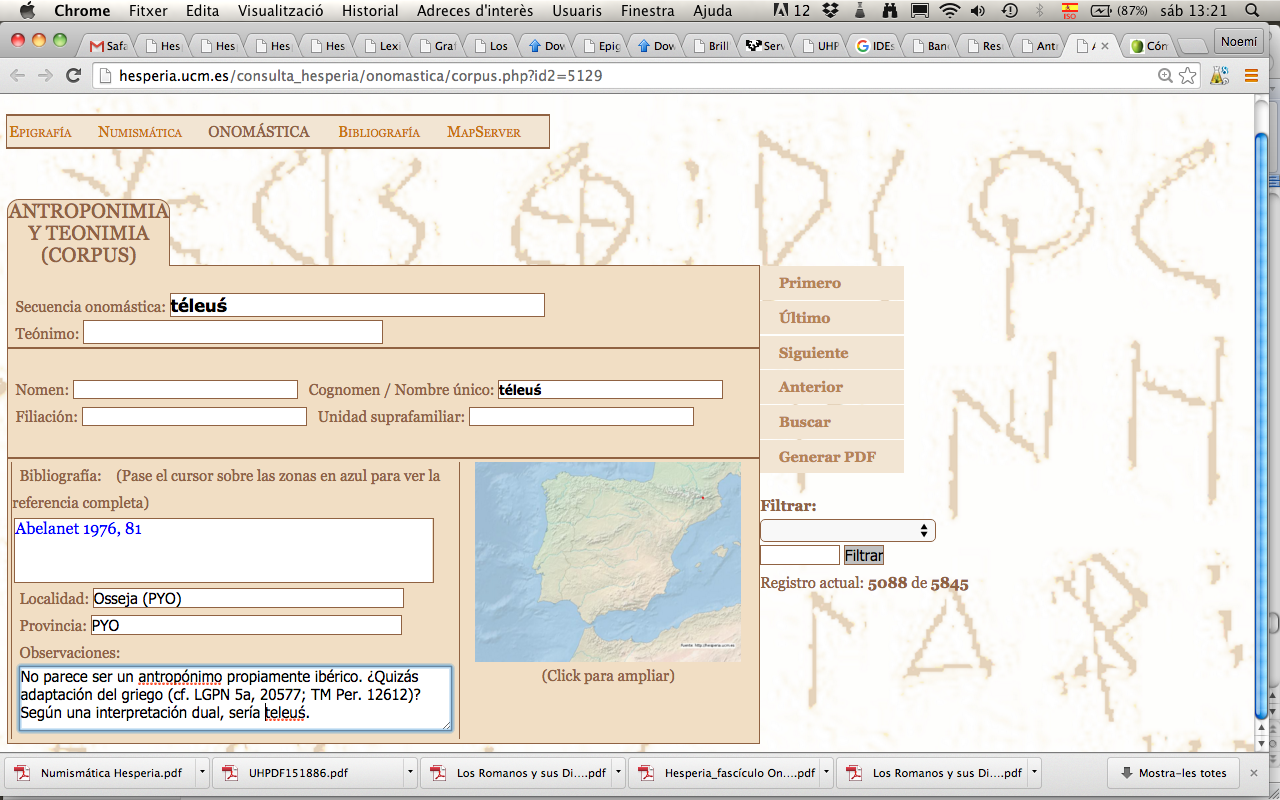
\includegraphics[width=\columnwidth]{EpigraphyandonomasticsinHesperiadatabanktemplate-img010.png}
\caption{Fig. 10: record of a possible Greek name attested in an Iberian inscription.}
\label{fig:10}
\end{figure}
 



A similar consideration might also apply, for instance, to another important document in the Palaeohispanic epigraphic
landscape, namely the III Botorrita Bronze plaque, written in Celtiberian language and script but containing a
considerable amount of foreign names, such as Latin or Greek.\footnote{ Vid. Unterman’s proposal in MLH IV, K.1.3. }
This could be the case for \emph{markos} (\emph{Marcus}), \emph{bolora} (\emph{Flora}), \emph{kinbiria} (\emph{Cimbria}), \emph{antiokos} (\emph{Antiochus}), \emph{bilinos}
(\emph{Philinus}), \emph{bilonikos} (\emph{Philonicus}), \emph{tais} (\emph{Thais}), \emph{tiokenes} (\emph{Diogenes}), and so on. We could finally mention, in this
same regard, the Gaullish names observed in some Iberian inscriptions from southern France: \emph{aśetile} (\emph{Adsedilus}, CIL III
5373), \emph{tesile} (\emph{Tessillus}, CIL III 14368.28), \emph{uaśile} (\emph{Vassil(l)us}, CIL XII 2286), \emph{katubaŕe} (\emph{Catumarus}, CIL 3, 4263),
etc.

To sum up, the new dynamic sections of Hesperia provide an essential boost to a field of study, the detection of
anthroponymic areas, which, thanks to the previous work by M. Gómez Moreno and J. Untermann, has been proved to be very
productive for the comprehension of the linguistic diversity of the ancient Iberia. The study of the indigenous
languages on the basis of the distribution of their personal names is actually essential, sometimes even the only
available means, for the definition of these areas that remained anepigraphic in pre-Roman times (see the map in fig.
2, with the dispersal areas of Palaeohispanic inscriptions). Obviously, one of the main advantages of the digital
format is that it offers the possibility to regularly update the corpus with new data. However, the most remarkable
difference from a traditional corpus is that it allows the user to connect and freely cross the information, and to
project the results automatically on a map, which makes this a powerful resource for new research and new results.


CTS = Canonical Text Services (protocol to cite digitally-available texts in a canonical way).

EAGLE = The Europeana network of Ancient Greek and Latin Epigraphy:  \url{http://www.eagle-network.eu/}

IDEs = Integrating Digital Epigraphies project.

LGPN = The Lexicon of Greek Personal Names: \url{http://www.lgpn.ox.ac.uk/}

Pleiades = A community-built gazetteer and graph of ancient places: \url{http://pleiades.stoa.org/}

SNAP = Standards for Networking Ancient Prosopographies project: \url{http://snapdrgn.net/}

Trismegistos = Interdisciplinary portal of papyrological and epigraphical resources formerly Egypt and the Nile valley
(800 BC-AD 800): \url{http://www.trismegistos.org/}

\nocite{moncunill_ochocientos_????}
\nocite{untermann_monumenta_1975}
\nocite{vallejo_antroponimia_????}

\bibliographystyle{sapauth-eng}
\bibliography{../../EAGLE}

\end{document}
